%; whizzy chapter
% -initex iniptex -latex platex -format platex -bibtex jbibtex -fmt fmt
% 以上 whizzytex を使用する場合の設定。

%     Tokyo Debian Meeting resources
%     Copyright (C) 2011 Junichi Uekawa
%     Copyright (C) 2011 Nobuhiro Iwamatsu

%     This program is free software; you can redistribute it and/or modify
%     it under the terms of the GNU General Public License as published by
%     the Free Software Foundation; either version 2 of the License, or
%     (at your option) any later version.

%     This program is distributed in the hope that it will be useful,
%     but WITHOUT ANY WARRANTY; without even the implied warranty of
%     MERCHANTABILITY or FITNESS FOR A PARTICULAR PURPOSE.  See the
%     GNU General Public License for more details.

%     You should have received a copy of the GNU General Public License
%     along with this program; if not, write to the Free Software
%     Foundation, Inc., 51 Franklin St, Fifth Floor, Boston, MA  02110-1301 USA

%  preview (shell-command (concat "evince " (replace-regexp-in-string "tex$" "pdf"(buffer-file-name)) "&"))
% 画像ファイルを処理するためにはebbを利用してboundingboxを作成。
%(shell-command "cd image201201; ebb *.png")

%%ここからヘッダ開始。

\documentclass[mingoth,a4paper]{jsarticle}
\usepackage{monthlyreport}
\usepackage{alltt}

\newcommand{\commandannotate}[2][4]{%
  \raisebox{0.33ex}{%
    \smash{%
      \ovalbox{%
        {\scriptsize\rule{0pt}{0.75ex}}%
        \smash{%
          \raisebox{-0.25ex}{%
            \scriptsize{}%
            \ifcase#1%           0
            \or $\uparrow{}$%    1
            \or $\rightarrow{}$% 2
            \or $\downarrow{}$%  3
            \or $\leftarrow{}$%  4
            \else%               5-9
            \fi%
            {#2}%
          }%
        }%
      }%
    }%
  }%
}
\newenvironment{terminal}{%
  \begin{trivlist}\item\begin{screen}%
    \begin{alltt}\renewcommand{\baselinestretch}{0.75}%
      \begin{small}%
}{%
      \end{small}%
    \end{alltt}%
  \end{screen}\end{trivlist}%
}

% 日付を定義する、毎月変わります。
\newcommand{\debmtgyear}{2012}
\newcommand{\debmtgmonth}{3}
\newcommand{\debmtgdate}{17}
% (+ (* (- 2012 2005) 12) 3 -1) started from zero
\newcommand{\debmtgnumber}{86}

\begin{document}

\begin{titlepage}
\thispagestyle{empty}
% タイトルページ:編集必要な部分は最初のマクロに飛ばすこと

\vspace*{-2cm}
第\debmtgnumber{}回 東京エリア Debian 勉強会資料\\
\hspace*{-2cm}

\includegraphics[width=210mm]{image201003/debsen.eps}\\
\hfill{}\debmtgyear{}年\debmtgmonth{}月\debmtgdate{}日

% ここはアップデートすること
% 全角文字にしないとフォントのサイズが合わないので注意
\rotatebox{10}{\fontsize{32}{32} {\gt Debian 勉強会 -ユーザサイド-}}

\rotatebox{10}{\fontsize{32}{32} {\gt Apache2 / HTTP サーバから始める Debian}}

\vspace*{-2cm}
\hfill{}
\includegraphics[height=6cm]{image200502/openlogo-nd.eps}
\end{titlepage}

\dancersection{Introduction}{上川 純一}

\begin{multicols}{2}
 

 今月のDebian勉強会へようこそ。これからDebianの世界にあしを踏み入れると
 いう方も、すでにどっぷりとつかっているという方も、月に一回Debianについ
 て語りませんか?

 Debian勉強会の目的は下記です。

 \begin{itemize}
 \item \underline{Debian Developer} (開発者)の育成。
 \item 日本語での「\underline{開発に関する情報}」を整理してまとめ、アップデートする。
 \item \underline{場}の提供。
 \begin{itemize}
  \item 普段ばらばらな場所にいる人々が face-to-face で出会える場を提供
	する。
  \item Debian のためになることを語る場を提供する。
  \item Debianについて語る場を提供する。
 \end{itemize}
 \end{itemize}		

 Debianの勉強会ということで究極的には参加者全員がDebian Packageをがりがり
 と作るスーパーハッカーになった姿を妄想しています。情報の共有・活用を通し
 て Debianの今後の能動的な展開への土台として、「場」としての空間を提供す
 るのが目的です。

\end{multicols}

\newpage

\begin{minipage}[b]{0.2\hsize}
 \definecolor{titleback}{gray}{0.9}
 \colorbox{titleback}{\rotatebox{90}{\fontsize{80}{80} {\gt デビアン勉強会} }}
\end{minipage}
\begin{minipage}[b]{0.8\hsize}
\hrule
\vspace{2mm}
\hrule
\begin{multicols}{2}
\tableofcontents
\end{multicols}
\vspace{2mm}
\hrule
\end{minipage}

\dancersection{最近のDebian関連のミーティング報告}{岩松 信洋}
\subsection{東京エリアDebian勉強会85回目報告}

\subsection{福岡Debian勉強会0回目報告}
たまたま 福岡に行く機会がありましたで、2012年2月18日に 福岡で 第0回 福岡Debian勉強会
を行いました。
岩松が DKMS の仕組みと Debianでの対応状況、パッケージ作成方法について説明しました。
いきなりカーネルの話をするので、参加者はちょっと引いていました。
DKMS へサポート体制はほとんど完了しており、ユーザは容易に使えることが分かりました。
Debianパッケージ化をサポートするツールもあるので、まだDKMSをサポートしていないしてない
メンテナはサポートしましょう。

また、山田さんが Debianサーバを容易に量産する仕組みについて紹介しました。
いかに速く「構築」できるか、楽に「構築」できるか いかに楽に「再現」できるかについて
紹介し、 Debianにはこれらを満たすツールがたくさんあることが分かりました。
ユーザランドイメージ作るなら、debootstrap ではなく、multistrap 
を使うのがよいそうです。
第1回は未定ですが、今後も福岡でのDebian勉強会開催が期待されます。

% (query-replace-regexp "<.*?>" "")
% (query-replace-regexp "^[	 ]\+" "")

\dancersection{Debian 勉強会 - ユーザサイド -  Apache2 / HTTP サーバから始める Debian}{岩松 信洋}

普段はちょっと開発者寄りな話をしているDebian
勉強会ですが、今回は OSC 出張企画として、ユーザー視点の勉強会を開催します。
今回はよく使われていると思われる Apache2 / HTTP サーバ に焦点を当ててみます。

\subsection{はじめに}

Debian は 日本では HTTP サーバとして利用されているように見えませんが、
世界では一番採用されている Linux ディストリビューションになったようです。
\footnote{\url{http://w3techs.com/blog/entry/debian_is_now_the_most_popular_linux_distribution_on_web_servers}}
この記事によると、利用されている理由は HTTP サーバパッケージの種類が多くある事が理由の一つに挙げられています。
Debian を HTTP サーバとして利用している理由を実際に使っている方に聞いてみたところ、理由はこれだけではないことが分かりました。
Debianのパッケージングシステム、APT、Apahce モジュールパッケージの多さ、
Webアプリケーションで採用される P言語(Perl, Python, PHP)のサポートなどがあり、
一番良い点として挙げられたのは設定ファイルの柔軟性についてでした。

Debian の Apache2 / HTTP サーバ は Red Hat 系 と違い、Debian 特有の構成になっています。これは他のディストリビューションしか
知らない人にとっては難しいかもしれません。
しかしDebian特有の構成を理解すると、他のディストリビューションとのメリット、
デメリットが見えてくると思います。
というわけで今回は、Debian の Apache2 / HTTP サーバ (以下、Apache2 ) について勉強していこうと思います。

\subsection{Debian の Apache2 バージョン}

まず、Debian で提供されている Apache2 のバージョンを見てみます。
表\ref{tab:apache-version}にまとめました。
Upstream と比べると少し古いですが、機能的には問題ないでしょう。
RHEL、CentOS(\texttt{バージョン 2.2.15-15})
と比べても特にバージョンが古いというわけでもありません。

\begin{table}[ht]
\begin{center}
\begin{tabular}{|l|l|l|l|l|l|}
\hline 
ディストリビューション & stable & testing &unstable & experimental & upstream\\
\hline \hline
バージョン & 2.2.16-6+squeeze6 & 2.2.22-1 & 2.2.22-1 & - & 2.4.1 \\
\hline
\end{tabular}
\caption{\label{tab:apache-version}Debian ディストリビューションと Apache2 のバージョン}
\end{center}
\end{table}

\subsection{Debianのパッケージ構成とパッケージのインストール}

次に Apache2 のパッケージ構成とインストール方法について説明します。

\subsubsection{パッケージ構成}

Debian の Apache2 で提供されているパッケージは以下の通りです。
HTTP サーバの処理モデルごとにパッケージ
(apache2-mpm-worker、apache2-mpm-prefork、apache2-mpm-event、apache2-mpm-itk)
が分離されていることがわかります。
これにより自分の用途に合わせたパッケージをインストールできます。
Red Hat系は一つのパッケージに纏まっていて、処理モデル毎にサフィックスをつけています(例:httpd.worker)。
\begin{table}[ht]
\begin{center}
\begin{tabular}{|l|l|}
\hline 
パッケージ名 & パッケージの説明\\
\hline \hline 
apache2 & Apache HTTP サーバメタパッケージ \\
\hline
apache2-mpm-worker & スレッドモデル Apche HTTP サーバ\\
\hline 
apache2-mpm-prefork & 非スレッドモデル Apache HTTP サーバ\\ 
\hline
apache2-mpm-event & イベントドリブンモデル Apache HTTP サーバ\\ 
\hline 
apache2-mpm-itk & マルチユーザ環境  Apache HTTP サーバ\\
\hline
apache2.2-common & Apache HTTP サーバ 共通ファイル \\
\hline
apache2.2-bin & Apache HTTP サーバの共通バイナリファイル\\ 
\hline
apache2-utils & ウェブサーバ用ユーティリティプログラム \\
\hline
apache2-suexec & Apache2 mod-suexec 用 基本 suexec プログラム \\
\hline
apache2-suexec-custom & Apache2 mod-suexec 用 設定可能 suexec プログラム \\
\hline
apache2-dbg & Apache HTTP サーバ デバッグシンボルファイル \\
\hline
apache2-prefork-dev & 非スレッドモデル Apache HTTP サーバ 開発用ヘッダファイル\\
\hline
apache2-threaded-dev & マルチスレッドモデル Apache HTTP サーバ 開発用ヘッダファイル \\
\hline
apache2-doc & Apache HTTP サーバドキュメント \\
\hline
\end{tabular}
\caption{\label{tab:apache-pkg}Debian で 提供される Apache2 パッケージ}
\end{center}
\end{table}

次にパッケージの依存関係図を図\ref{tab:apache-pkg}に示します。依存関係が複雑なので
ユーザは不安になるかもしれません。しかしDebianでは
強力なパッケージ管理ツール APT によって気にする事なくインストールできます。

\begin{figure}[ht]
 \begin{center}
  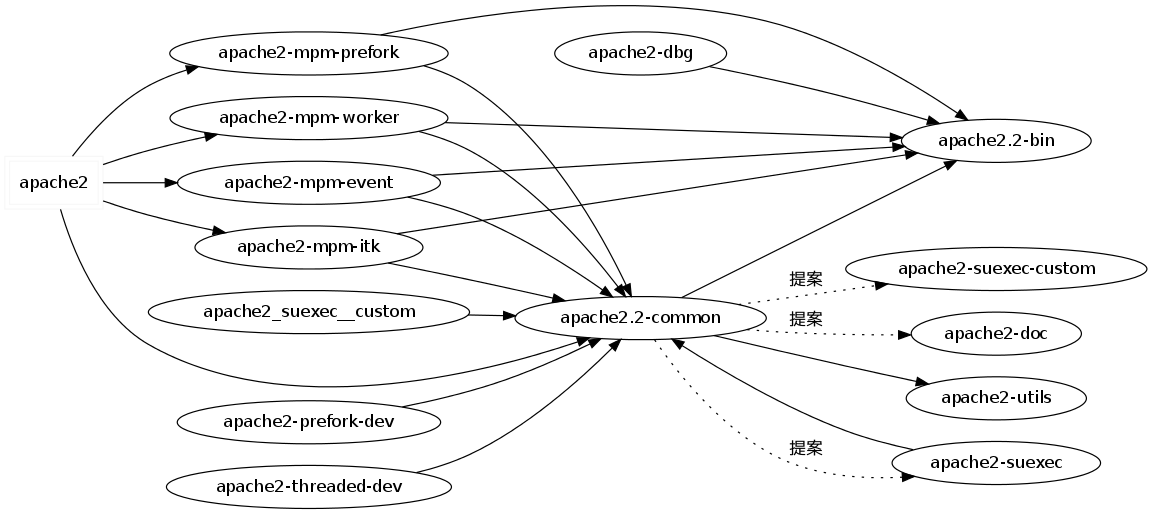
\includegraphics[width=1.0\hsize]{image201203/apache2-pkg.png}
 \end{center}
\label{tab:apache-pkg}\caption{Debian でのパッケージ依存関係}
\end{figure}

\subsubsection{インストール}

Debianで Apache2 をインストールする場合は \texttt{apt-get install}コマンドを
使います(図\ref{fig:install})。

Debianでは apache2 というメタパッケージを使ってインストールすることが多いです。
apache2 をインストールすると、apache2-mpm-worker がインストールされます。
他の HTTP サーバパッケージをインストールしたい場合は、各々のパッケージを
指定してインストールする必要があります。

またCentOSなどでは、「httpd」 パッケージとして提供されているのでパッケージ名が異なります。
普段は他のディストリビューションを使っている人は注意しましょう。


\begin{figure}[ht]
 \begin{center}

\begin{terminal}
$ sudo apt-get update \commandannotate{リポジトリを更新}
$ sudo apt-get install apache2 \commandannotate{apache2 パッケージをインストール}
\end{terminal}

 \end{center}
\label{fig:install}\caption{Debian で Apache2 をインストールする}
\end{figure}


\subsubsection{Apache HTTP サーバの起動と停止}

Debian は「インストールしたものは使う」というポリシーなので、インストール完了の時点で
既に Apache HTTP サーバは起動しています。停止したい場合には root 権限で 
「\texttt{/etc/init.d/apache2 stop}」 を実行します。
起動したい場合は 「\texttt{/etc/init.d/apache2 start}」、再起動したい場合には
「\texttt{/etc/init.d/apache2 restart}」を実行します。
図\ref{fig:startstop}に例を示します。

\begin{figure}[ht]

\begin{terminal}
$ ps ax | grep apache2 \commandannotate{apache2 のプロセスを確認}
10034 ?        Ss     0:05 /usr/sbin/apache2 -k start
13008 ?        S      0:00 /usr/sbin/apache2 -k start
....
$ sudo /etc/init.d/apache2 stop \commandannotate{apache2 を停止}
$ ps ax | grep apache2 \commandannotate{apache2 のプロセスを確認}
16833 pts/1    S+     0:00 grep apache2 
$ sudo /etc/init.d/apache2 start \commandannotate{apache2 を開始}
10048 ?        Ss     0:05 /usr/sbin/apache2 -k start
13024 ?        S      0:00 /usr/sbin/apache2 -k start
....
\end{terminal}

\label{fig:startstop}\caption{Apache2の起動と停止}
\end{figure}



デフォルトの状態では、マシンを立ち上げ時に HTTP サーバが起動するようになっています。
マシン立ち上げ時に HTTP サーバの起動しないようにするには、ランレベル毎のサービス起動スクリプト
を制御するツール \texttt{update-rc.d}を使います。

全てのランレベルで apache2 を起動させないようにするには、コマンドに
サービス名と remove を指定して実行します。 

またインストール直後のデフォルトの状態に戻したい場合には、コマンドに
サービス名と default を指定して実行します。

実行例を図\ref{fig:update-rc}に示します。


\begin{figure}[ht]
\begin{terminal}
$ sudo update-rc.d -f apache2 remove \commandannotate{全てのランレベルで apache2 を起動させないようにする。} 
$ sudo update-rc.d -f apache2 default \commandannotate{サーバ起動をデフォルトの状態に戻す}
\end{terminal}
%$
\label{fig:update-rc}\caption{ランレベルの制御}
\end{figure}


Red Hat系では \texttt{chkconfig}を使いますが、Debianでも提供されています。
しかし、chkconfig は RedHat系のサービス管理ツールなので Debian 
ではうまく動作しないことがあるようです。同様のツールとして
\texttt{sysv-rc-conf}があるのでこちらを使ったほうがいいでしょう。
図\ref{fig:sysv-rc}に簡単な使い方を説明します。

\begin{figure}[ht]

\begin{terminal}
$ sudo apt-get install sysv-rc-conf \commandannotate{sysv-rc-conf パッケージをインストール} 
$ sudo sysv-rc-conf --list  \commandannotate{現在の状態を出力}
apache2      0:off1:off2:on3:on4:on5:on6:off
bootlogd     S:on
(中略)
$ sudo sysv-rc-conf --level 2 apache2 off \commandannotate{ランレベル2のapache2を無効にする}
$ sudo sysv-rc-conf --list | head -1 \commandannotate{現在の状態を出力}
apache2      0:off1:off2:off3:off4:off5:off6:off
$ sudo sysv-rc-conf --level 2 apache2 on\commandannotate{ランレベル2のapache2を有効にする} 
$ sudo sysv-rc-conf --list | head -1  \commandannotate{現在の状態を出力}
apache2      0:off1:off2:on3:off4:off5:off6:off
\end{terminal}
%$
\label{fig:sysv-rc}\caption{Apache2の起動と停止}
\end{figure}


\subsection{Apache2 の設定ファイル}

Red Hat 系の場合、主な設定は \texttt{/etc/httpd/conf/httpd.conf}で行い、include されるファイルは
\texttt{/etc/httpd/conf.d/}ディレクトリに格納しますが、Debian の場合は表\ref{tab:apache-files}のように
なっています。

\begin{table}[ht]
\begin{center}
\begin{tabular}{|l|l|}
\hline 
設定ファイル & 内容\\
\hline \hline
/etc/apache2/apache2.conf & 基本設定\\
\hline
/etc/apache2/httpd.conf & オーバーライドする設定\\
\hline
/etc/apache2/conf.d/ & 基本設定の中でIncludeするファイルを格納する\\
\hline
/etc/apache2/ports.conf & ポートの設定\\
\hline
/etc/apache2/envvars & 環境変数の設定\\
\hline
/etc/apache2/mods-available/ & 利用可能なモジュール設定\\
\hline
/etc/apache2/mods-enabled/ & 利用中のモジュール設定\\
\hline
/etc/apache2/sites-available/ & 利用可能なサイト設定\\
\hline
/etc/apache2/sites-enabled/ & 利用中のサイト設定\\
\hline
/var/www & ドキュメントルート\\
\hline
/usr/lib/cgi-bin & cgi-bin\\
\hline
/var/log/apache2 & Apache2 ログ\\
\hline
\end{tabular}
\caption{\label{tab:apache-files}{Debian の Apache2 設定ファイル群}}
\end{center}
\end{table}

\texttt{apache2.conf}には図\ref{fig:apache2conf}のような行があり、\texttt{apache2.conf}
から各設定が読み込まれるようになっています。
Apache2 の設定を
を変更する場合、\texttt{apache2.conf}を変更せず、
\texttt{httpd.conf} や \texttt{ports.conf}を変更します。

\begin{figure}[ht]
\begin{terminal}
(省略)
# Include module configuration:
Include /etc/apache2/mods-enabled/*.load
Include /etc/apache2/mods-enabled/*.conf

# Include all the user configurations:
Include /etc/apache2/httpd.conf

# Include ports listing
Include /etc/apache2/ports.conf
(中略)
# Include generic snippets of statements
Include /etc/apache2/conf.d/

# Include the virtual host configurations:
Include /etc/apache2/sites-enabled/
\end{terminal}

\label{fig:apache2conf}\caption{apache2.confの内容}
\end{figure}


\subsection{サイトを設定する}

Debian は\texttt{/etc/apache2/sites-available/default} に apache2 のデフォルトのサイト設定
を格納しています。サイトを一つだけ構築する場合はこのファイルを変更し、
apache2 を再起動すれば
設定された内容で apache2 が立ち上がります。再起動する方法は図\ref{fig:apache2restart}の通りです。

\begin{figure}[ht]
\begin{terminal}
$ sudo /etc/init.d/apache2 restart
\end{terminal}
%$
\label{fig:apache2restart}\caption{Apache2の再起動}
\end{figure}

Debian の apache2 で複数のサイトを立ち上げる場合、httpd.conf や apache2.conf は編集しません。
サイト別に設定を記述し、\texttt{/etc/apache2/sites-available/}ディレクトリに格納します。
そして、そのサイトを設定を有効にするコマンド「\texttt{a2ensite}」実行し、apache2 を再起動します。

簡単な手順を説明します。
例えば、test.example.org というサイトを立ち上げるとします。内容は図\ref{fig:siteexample}のようになるでしょう。

\begin{figure}[ht]
\begin{terminal}
<VirtualHost *>
    ServerAdmin admin-test@example.org
    ServerName test.example.org
    DocumentRoot /home/test/public_html/
    <Directory />
        Options FollowSymLinks ExecCGI Includes
        AllowOverride None
    </Directory>
</VirtualHost>
\end{terminal}
\label{fig:siteexample}\caption{サイトの設定例}
\end{figure}


そしてこのサイト設定を\texttt{/etc/apache2/sites-available/test}に格納します。
格納した後、サイトを有効にする「\texttt{a2ensite}コマンド」に有効にしたいサイトの
設定ファイル名を指定して実行します。実行すると\texttt{/etc/apache2/sites-enabled/}
にシンボリックリンクが張られ設定が有効になります。
有効にしただけでは、稼働しているhttpd サーバには設定が反映されていないため、
httpd サーバを再起動します。

図\ref{fig:siteenable-setting}に例を示します。

\begin{figure}[ht]
\begin{terminal}
$ ls -l /etc/apache2/sites-enabled/
合計 0
lrwxrwxrwx 1 root root 26 2011-03-20 08:23 000-default -> ../sites-available/default
lrwxrwxrwx 1 root root 30 2011-03-20 08:23 default-ssl.old -> ../sites-available/default-ssl
$ sudo a2ensite test \commandannotate{test を有効にする}
Enabling site test.
Run '/etc/init.d/apache2 reload' to activate new configuration!
$ ls -l /etc/apache2/sites-enabled/
合計 0
lrwxrwxrwx 1 root root 26 2011-03-20 08:23 000-default -> ../sites-available/default
lrwxrwxrwx 1 root root 29 2012-03-10 06:24 test -> ../sites-available/test
lrwxrwxrwx 1 root root 30 2011-03-20 08:23 default-ssl.old -> ../sites-available/default-ssl
$ sudo /etc/init.d/apache2 restart \commandannotate{Apache2 を再起動}
\end{terminal}
\label{fig:siteenable-setting}\caption{サイトを有効にする}
\end{figure}

サイトの設定を無効にする場合には、サイトを有効にする「\texttt{a2dissite}コマンド」
に無効にしたいサイトの設定ファイル名を指定して実行します。実行すると\texttt{/etc/apache2/sites-enabled/}
からシンボリックリンクが削除されます。サイト設定を無効にした後は、有効時と同様にhttpd サーバを
再起動する必要があります
図\ref{fig:sitedisable-setting}に例を示します。

\begin{figure}[ht]
\begin{terminal}
$ sudo a2dissite test \commandannotate{test を無効にする}
Site test disabled.
Run '/etc/init.d/apache2 reload' to activate new configuration!
$ ls -l /etc/apache2/sites-enabled/
合計 0
lrwxrwxrwx 1 root root 26 2011-03-20 08:23 000-default -> ../sites-available/default
lrwxrwxrwx 1 root root 30 2011-03-20 08:23 default-ssl.old -> ../sites-available/default-ssl
\end{terminal}
%$

\label{fig:sitedisable-setting}\caption{サイトを無効にする}
\end{figure}

このように Debian ではサイトの設定を分離し、サイト毎に状態を管理することができます。
他のディストリビューションでは \texttt{include} 等を使って管理することができますが、
ファイル内容を変更する必要があり非常に手間です。
Debian はシンボリックリンクを使うことによってApache2 の設定ファイルを
変更せずにサイト設定の有効・無効ができるようになっています。

\subsection{モジュールを有効/無効にする}
Debian のモジュールに関する設定はモジュール毎の設定ファイルとして
\texttt{mods-available}ディレクトリに格納されています。
それらのうち、実際に有効にするものが
シンボリックリンクとして \texttt{mods-enabled} ディレクトリに張られます。
シンボリックリンクは手動で行わず、モジュールを有効にする場合には\texttt{a2enmod}コマンド、
無効にする場合には\texttt{a2enmod}コマンドを使います。

図\ref{fig:a2enmod}にmod\_info を有効にする例を、
図\ref{fig:a2dismod}にmod\_info を有効にする例を示します。

\begin{figure}[ht]
\begin{terminal}
$ 
sudo a2enmod info
\end{terminal}
%$
\label{fig:a2enmod}\caption{mod\_infoを有効にする}
\end{figure}

\begin{figure}[ht]
\begin{terminal}
$ sudo a2dismod info
\end{terminal}
%$
\label{fig:a2dismod}\caption{mod\_infoを無効にする}
\end{figure}

\subsection{その他}

その他、注意すべき点をいくつか教えてもらったので紹介します。

\subsubsection{libapache2-mod-php5 と apache2-mpm-prefork}

Apache2 上で mod-php5 を使いたい場合、apache2-mpm-worker は使えない点に
注意してください。これは PHP5(mod-php5)の制限で、スレッドで動作することができないためです。
libapache2-mod-php5 をインストールすると、
を使いたい場合、apache2-mpm-worker が削除され、apache2-mpm-prefork がインストールされます。
PHP ユーザの方は注意しましょう。

\subsubsection{再起動確認について}
その他、Debian で Apache2 を使う理由として、再起動確認を行うという点があります。
例えばglibc が更新されたとき、サーバ系は再起動する必要があるのですが、Red Hat系では
再起動してくれず、管理者が手動で行う必要があります。
CentOS を使っている会社ではデーモンを再起動しないとならないアップデートがあったかどうか
チェックするツールをわざわざ作って管理していたりするようです。
しかし Debian では再起動の確認が行われる(設定によって自動再起動も可能)ので、
管理者の手を煩わせません。このような細かいところに気を使ってくれるのも Debianの良い所です。

\subsection{まとめ}

Debian のパッケージ古いというのは昔の話。
セキュリティ対応あるし、早い。
Debian の設定ファイルが独自なのは理由がある。
専用のツールもあるので、慣れるとメンテナンスが容易。
パッケージによる、細かいところへの気配り。
とりあえず、Debian 使え。

\printindex

\cleartooddpage

\vspace*{15cm}
\hrule
\vspace{2mm}

\includegraphics[width=2cm]{image200502/openlogo-nd.eps}
\noindent \Large \bf Debian 勉強会資料\\
\noindent \normalfont \debmtgyear{}年\debmtgmonth{}月\debmtgdate{}日 \hspace{5mm}  初版第1刷発行\\
\noindent \normalfont 東京エリア Debian 勉強会 (編集・印刷・発行)\\
\hrule

\end{document}
